\documentclass{article}
\usepackage{graphicx} % Required for inserting images
\usepackage[backend=biber, style=ieee]{biblatex}
\addbibresource{references.bib}
\usepackage[
    top=2cm,
    bottom=2cm,
    left=2cm,
    right=2cm
]{geometry}
\usepackage{booktabs}
\usepackage{float}
\usepackage{amsmath}
\usepackage[hidelinks]{hyperref}
\usepackage{subcaption}

\title{
\Huge Big Data Analytics \\
\vspace{0.5em}
\Large{Real-time Financial Transaction Anomaly Detection}}

\author{Julia Kruk, Barbara Seweryn, Zuzanna Sieńko, Nadia Serafin}
\date{}

\begin{document}
\maketitle

\newpage
\tableofcontents

\newpage

\section{Project overview}
The objective of this project is to design and implement a real-time financial transaction minitoring and unsupervised anomaly detection system using Big Data technologies and machine learning.

The solution will follow a Lambda Architecture. It will combine three different data sources including batch processing of historical financial transactions and stream processing of incoming transaction events. Additionally, synthetically generated account activity data, including login events and device information, will be incorporated to provide more detailed context for anomaly detection. A data generation and ingestion component will publish transaction and account activity events to Apache Kafka, while the data will be stored in MinIO storage.

The batch layer will be responsible for training machine learning models on historical data and periodically retraining them as new data becomes available. In parallel, the speed layer will perform streaming inference by processing incoming transactions, applying the necessary preprocessing, and using latest trained model to generate anomaly risk prediction. Data processed in batch and speed layers will be available as real-time and batch views using Cassandra.

The results will be presented through an interactive dashboard using Streamlit. It will allow users to monitor transaction activity, investigate anomaly alerts and explore statistics related to user behaviour.

\section{Project deliverables from user's perspective}
From the user's perspective, the system will provide the following functionalities:
\begin{enumerate}
    \item Real-time transaction monitoring -- users will be able to observe incoming financial transactions and their anomaly risk prediction.
    \item Anomaly detection and alerts -- transactions identified as suspicious will be highlighted and presented in a dedicated alert section, drawing users' attention to those suspicious activities.
    \item Transaction investigation and statistics -- users will be able to examine individual transactions and explore overall transaction activity through interactive visualisations. The dashboard will present statistics such as transaction volumes, average transaction amounts, transaction type distributions, and transaction trends over time.
    \item Anomaly detection analytics and model performance -- users will be able to analyze the results of the anomaly detection system, including alert trends over time. The dashboard will also provide model performance metrics, such as confusion matrices, precision, recall, and F1-score.
\end{enumerate}

\section{Project diagram with core use-cases}

\section{Data sources and their preliminary investigation}
\subsection{PaySim -- financial transaction dataset}
PaySim is a synthetic dataset available on Kaggle: \href{https://www.kaggle.com/datasets/ealaxi/paysim1}{Synthetic Financial Datasets For Fraud Detection} simulating mobile money transactions, generated based on real transaction patterns from a financial service provider. It contains 6 362 620 records and 11 features. Those features and their types are as follow:
\begin{table}[H]
    \centering
    \caption{Data types of the PaySim dataset attributes}
    \label{tab:paysim_dtypes}
    \begin{tabular}{ll}
        \toprule
        \textbf{Attribute} & \textbf{Data type} \\
        \midrule
        step & int64 \\
        type & categorical \\
        amount & float64 \\
        nameOrig & string \\
        oldbalanceOrg & float64 \\
        newbalanceOrig & float64 \\
        nameDest & string \\
        oldbalanceDest & float64 \\
        newbalanceDest & float64 \\
        isFraud & int64 \\
        isFlaggedFraud & int64 \\
        \bottomrule
    \end{tabular}
\end{table}
One simulation step represents one hour, with 743 observed steps spanning approximately 31 days. \\
The dataset contains two fraud-related fields: isFraud, identifying fraudulent transactions in the simulation, and isFlaggedFraud, representing an existing rule-based detection mechanism. Since the project focuses on unsupervised anomaly detection rather than supervised fraud classification, these labels will not be used as model input features or training targets. The objective is to identify transactions that deviate from typical patterns. \\

Preliminary exploratory data analysis (EDA) revealed no missing values or duplicate records. The dataset contains five transaction types:
\begin{itemize}
    \item CASH\_OUT -- 35.17\% of all transactions,
    \item PAYMENT -- 33.81\% of all transactions,
    \item CASH\_IN -- 22.00\% of all transactions,
    \item TRANSFER -- 8.38\% of all transactions,
    \item DEBIT -- 0.65\% of all transactions.
\end{itemize}
Transaction amounts are right-skewed, with a median of approximately 74 872 and a mean of 179 862. Significant differences in transaction amounts between transaction types suggest that transaction type should be considered when identifying unusual patterns.
\begin{figure}[H]
    \centering
    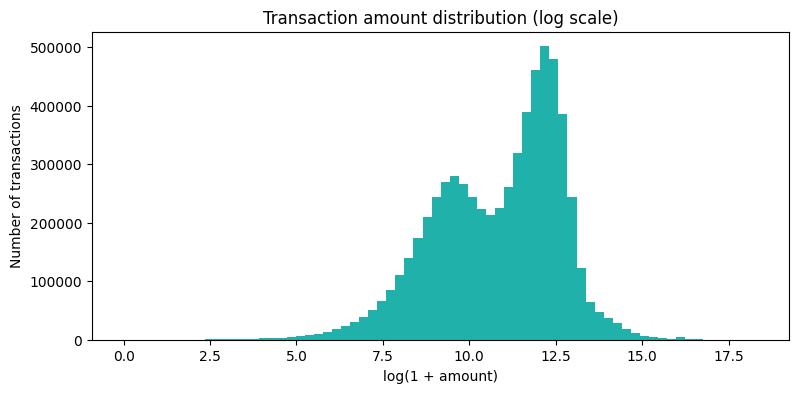
\includegraphics[width=0.8\textwidth]{report_plots/transaction_amount_dist.png}
    \caption{Distribution of transaction amounts (log scale)}
    \label{fig:transaction_types}
\end{figure}

Transaction activity varies over time, with hourly volumes ranging from 2 to 51 352 transactions. A substantial decrease in transaction volume is observed after approximately step 400, indicating a significant change in transaction activity patterns. To ensure that the historical dataset includes observations from both periods, the data will be divided some time after step 400th, e.g. at step 500. Transactions from the first 500 simulation hours will be used as historical batch data, while the remaining transactions will be replayed as a simulated stream. The aim of this approach is to allow the model to learn from different transaction activity patterns.
\begin{figure}[H]
    \centering
    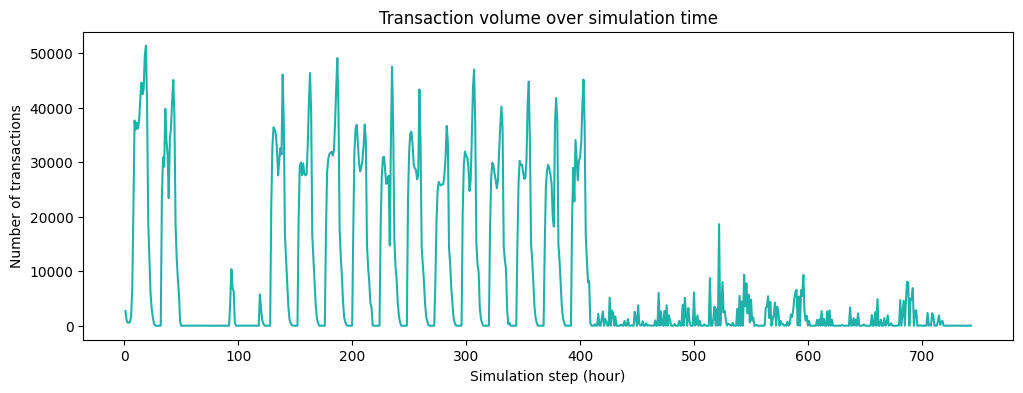
\includegraphics[width=0.8\textwidth]{report_plots/trans_volume_over_time.png}
    \caption{Transactions volume over time}
    \label{fig:trans_vol_over_time}
\end{figure}

The dataset contains 6 353 307 unique senders, indicating that nearly every sender appears only once. Only 814 streaming senders (0.27\%) also appear as senders in the historical dataset. Therefore, it is impossible to create individual sender profiles. Recipient identifiers show greater repetition, particularly for customer accounts (C), which receive an average of 7.36 transactions, compared with approximately one transaction per merchant (M). 
\begin{table}[H]
    \centering
    \caption{Customer and recipients transactions}
    \label{tab:C_R_transactions}
    \begin{tabular}{llll}
        \toprule
        \textbf{Recipient type} & \textbf{Transactions}  & \textbf{Unique recipients} & \textbf{Avg transactions per recipient}\\
        \midrule
        C & 4 211 125 & 571 961 & 7.36 \\
        M & 2 151 495 & 2 150 401 & 1.00 \\
        \bottomrule
    \end{tabular}
\end{table}
This suggests that historical recipient-level features may provide additional context, subject to their availability across the batch and streaming periods. Based on these findings, the proposed system will model typical transaction patterns rather than individual customer behavior.

\section{Infrastructure}
The solution will be based on Lambda architecture. 
\begin{itemize}
    \item Ingestion -- The system integrates 3 data sources: transactions from Bank X (sent in batches every hour), user activity data from Bank X (sent in batches every hour), and real-time transactions from Bank Y. Apache Kafka will serve as a message broker, routing the events to the next layers. The preprocessing component in the Speed layer and Storage component in the Batch layer will act as Kafka consumers.
    \item Batch layer -- Raw batch data will be stored in MinIO (or SeaweedFS) in Parquet format. Apache Airflow will orchestrate the process of retraining the machine learning model:
    \begin{itemize}
        \item Data will be loaded from the storage and preprocessed using Apache Spark;
        \item The ML model will be re-trained and saved back to the storage.
    \end{itemize}
    \item Speed layer -- The data will be preprocessed and the prediction will be generated using the latest model from the storage. This process will be handled by Apache Spark (or Kafka in Python). The data with the predictions will be sent to Serving layer.
    \item  Serving layer -- it will contain:
    \begin{itemize}
        \item Real-time views -- stored in Cassandra tables containing incoming transactions and their predictions;
        \item Batch views -- stored in Cassandra tables containing historical analysis and aggregations. 
    \end{itemize}
    \item Consumption -- The frontend part will be build using Streamlit. The user will be able to explore different views, such as real-time transaction monitoring or historical transaction statistics.
\end{itemize}

\section{Planned use of GenAI}
The use of GenAI tools will be limited to non-coding tasks.
Specifically, they will be used for:
\begin{itemize}
    \item help with research;
    \item styling the dashboard (e.g., CSS);
    \item debugging potential errors;
    \item grammar imporovement of the report, creating LaTex tables and diagrams.
\end{itemize}


\newpage
% ----------------------------  LIST OF FIGURES --------------------------------
\listoffigures
\thispagestyle{empty}

% -----------------------------  LIST OF TABLES --------------------------------
\renewcommand{\listtablename}{List of tables}
\listoftables
\thispagestyle{empty}

\end{document}